Las razones por las cuales se toma la decisión de fabricar la estructura del brazo mediante impresión 3D se detallan a continuación:

\begin{itemize}
  \item Cumplir con el requisito de replicabilidad y asequibilidad: Una de las bases del proyecto es que pueda ser reproducible a bajo coste tanto de recursos como de tiempo. Se decide por tanto construir la estructura física del brazo mediante técnicas de impresión 3D ya que están altamente extendidas y son cada vez mas asequibles.
  
  \item Características físicos del material: El plástico utilizado para la impresión es ligero y suficientemente resistente para soportar las cargas para las que esta pensado el manipulador.
  
  \item Disponibilidad de impresora 3D: Dado que la universidad es capaz de proveer al equipo con una impresora 3D funcional, los costes del proyecto se abaratan si realizamos la estructura con los medios de los que la universidad ya dispone.
  
  \item Simplificar el proceso de mejora y personalización: Debido a la naturaleza OpenSoftware y OpenHardware de nuestro proyecto esperamos que las personas puedan contribuir a el mejorándolo y/o personalizándolo. La impresión 3D facilita estas acciones.
\end{itemize}

Aprovechando la licencia GPL 3.0 hemos empleado el modelo 3D proporcionado por UFactory como punto de partida. A partir de este modelo se han impreso las piezas que hemos decidido conservar para nuestro proyecto.

\begin{figure}[H]
    \centering
    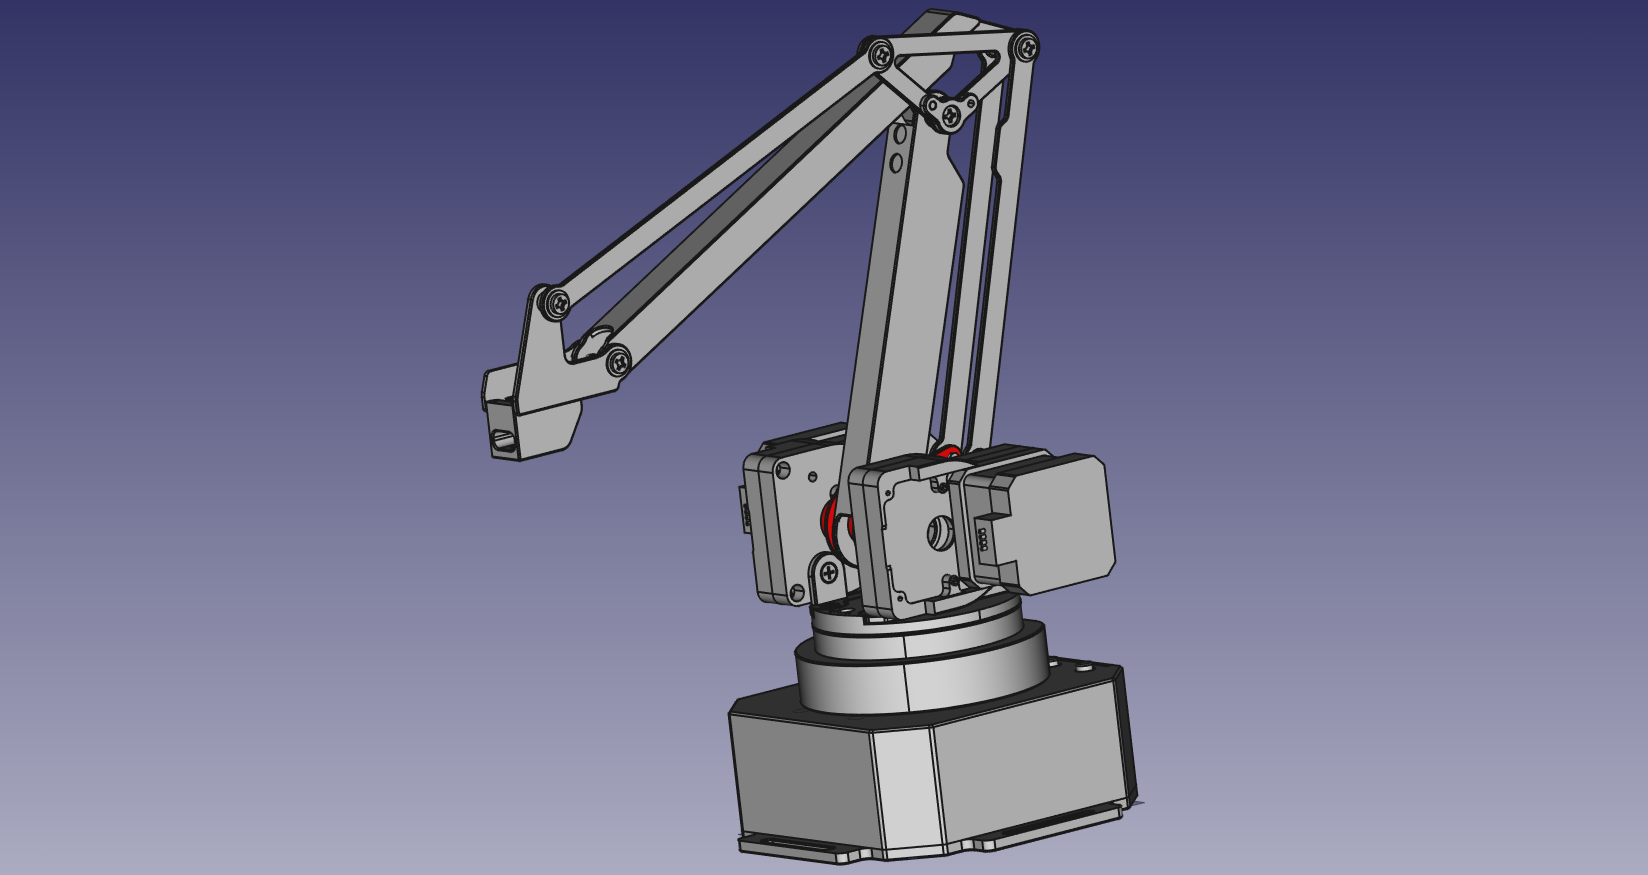
\includegraphics[width=12cm]{pictures/brazo_vista_3d_inicial.png}
    \caption{Concepto inicial del brazo robótico}
    \label{fig:manipulador_inicial}
\end{figure}

Las herramientas que hemos usado para visualizar y modificar el modelo y posteriormente imprimir las piezas han sido respectivamente FreeCAD y Slic3r.

\begin{figure}[H]
    \centering
    
\includegraphics[width=6cm]{pictures/freeCAD.jpg}
    
\includegraphics[width=6cm]{pictures/slic3r_logo.jpg}
    \caption{Herramientas utilizadas}
    \label{fig:herramientas_3d}
\end{figure}

El flujo de trabajo que se ha seguido desde el modelo 3D hasta la impresión de una pieza ha sido el siguiente.

\begin{figure}[H]
    \centering
    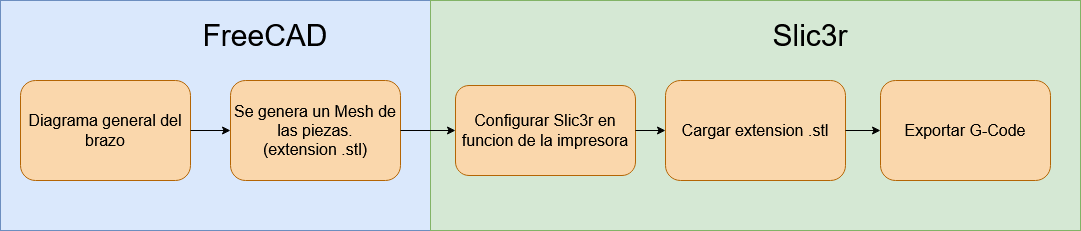
\includegraphics[width=.9\linewidth]{pictures/flujo_trabajo_impresion.png}
    \caption{Flujo de trabajo de la impresión 3D}
    \label{fig:flujo_3d}
\end{figure}

